\chapter{Mode~S meteorological services}

In the current Mode~S design, two message formats are used for aircraft to communicate meteorological conditions. These messages are meteorological routine air report (MRAR) and meteorological hazard report (MHR). In this chapter, we focus on explaining the information contained in these two types of messages.

\section{Meteorological routine air report (BDS 4,4)}

In MRAR messages, information on wind, air temperature, pressure, and humidity is transmitted. The structure of the message is shown in Table \ref{tb:bds44}.


\begin{table}[ht]
\renewcommand{\arraystretch}{1.1}
\centering
\caption{Meteorological routine air report (BDS 4,4), MB field}
\label{tb:bds44}
\begin{tabular}{|l|l|l|l|}
\hline
\textbf{FIELD} & \textbf{MSG} & \textbf{MB} & \textbf{BITS} \\ \hline
Figure of merit / source & 33-36 & 1-4 & 4 \\ \hline
Status (for wind) & 37 & 5 & 1 \\ \cdashline{1-1}
\begin{tabular}[c]{@{}l@{}}Wind speed\\ ~~\footnotesize Range: {[}0, 511{]} knots\\ ~~\footnotesize LSB: 1 knots\end{tabular} & 38-46 & 6-14 & 9 \\ \cdashline{1-1}
\begin{tabular}[c]{@{}l@{}}Wind direction\\ ~~\footnotesize Range: {[}0, 360{]} degrees\\ ~~\footnotesize LSB: 180/256 degrees\end{tabular} & 47-55 & 15-23 & 9 \\ \hline
Sign (for temperature) & 56 & 24 & 1 \\ \cdashline{1-1}
\begin{tabular}[c]{@{}l@{}}Static air temperature\\ ~~\footnotesize Range: {[}-128, +128{]} $^\circ$C\\ ~~\footnotesize LSB: 0.25 $^\circ$C \end{tabular} & 57-66 & 25-34 & 10 \\ \hline
Status (for pressure) & 67 & 35 & 1 \\ \cdashline{1-1}
\begin{tabular}[c]{@{}l@{}}Average static pressure\\ ~~\footnotesize Range: {[}0, 2048{]} hPa\\ ~~\footnotesize LSB: 1 hPa\end{tabular} & 68-78 & 36-46 & 11 \\ \hline
Status (for turbulence) & 79 & 47 & 1 \\ \cdashline{1-1}
Turbulence & 80-81 & 48-49 & 2 \\ \hline
Status (for humidity) & 82 & 50 & 1 \\ \cdashline{1-1}
\begin{tabular}[c]{@{}l@{}}Humidity\\ ~~\footnotesize Range: {[}0\%, 100\%{]} \\ ~~\footnotesize LSB: 100/64 \%\end{tabular} & 83-88 & 51-56 & 6 \\ \hline
\end{tabular}
\end{table}

The first field of the message defined the figure of merit (FOM) / source of the information. The values indicate the following:
\begin{itemize}
    \item 0: Invalid
    \item 1: Intertial system (INS)
    \item 2: Global Navigation Satellite System (GNSS)
    \item 3: Distance measuring equipment-based navigation (DME/DME)
    \item 4: Very High Frequency omnidirectional range / distance measuring equipment-based navigation (VOR/DME)
    \item 5-15: Reserved
\end{itemize}

For static air temperature, the encoded value can be negative. Hence, two's complement coding (see section \ref{sec:two_complement}) is used for decoding. The actual maximum range of temperature is from -80 $^\circ$C to +60 $^\circ$C.

It is also worth pointing out a discrepancy in the design. The temperature is encoded using 10 bits, where the least significant bit value should have been 0.125$^\circ$. However, according to the official document \cite{icao9871v1}, the LSB value is 0.25$^\circ$. ICAO has planned to update this to 0.125$^\circ$ in the future. Most current implementations still use 0.25$^\circ$. 

In Figure \ref{fig:bds44_example}, the decoding of an MRAR example message is shown.

\begin{figure}[ht]
    \centering
    

\tikzset{every picture/.style={line width=0.75pt}} %set default line width to 0.75pt        

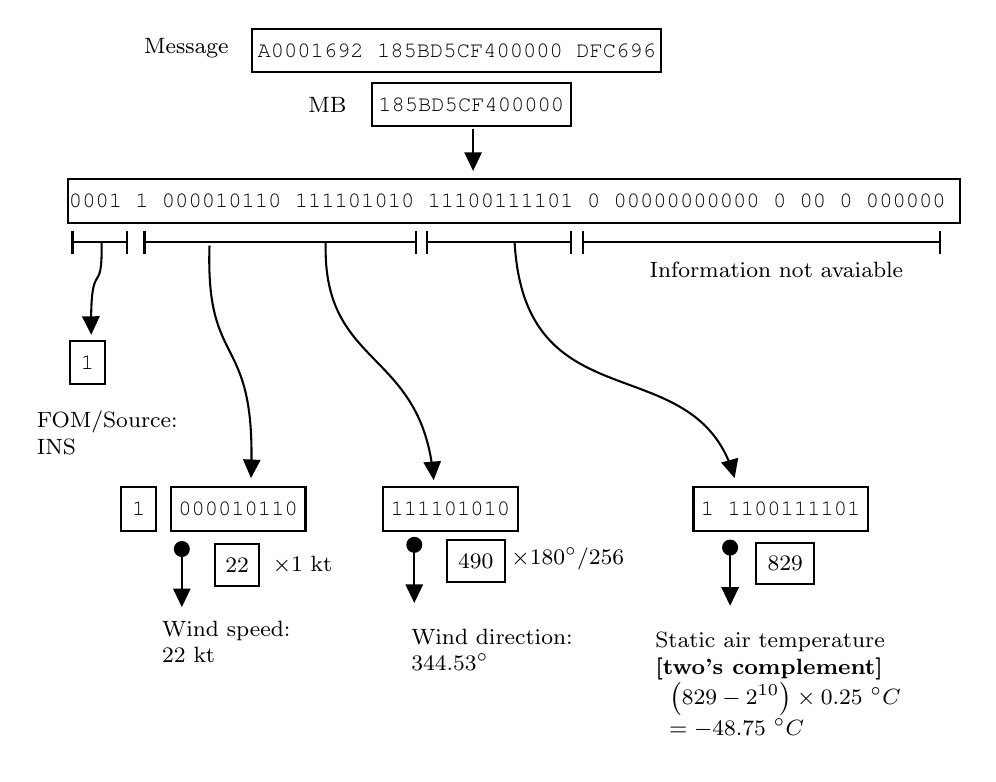
\begin{tikzpicture}[x=0.75pt,y=0.75pt,yscale=-1,xscale=1]
%uncomment if require: \path (0,402); %set diagram left start at 0, and has height of 402

%Curve Lines [id:da4469785122246488] 
\draw    (53,117.33) .. controls (53.57,145.77) and (47.64,122.56) .. (47.96,159.07) ;
\draw [shift={(48,162)}, rotate = 269.06] [fill={rgb, 255:red, 0; green, 0; blue, 0 }  ][line width=0.08]  [draw opacity=0] (8.93,-4.29) -- (0,0) -- (8.93,4.29) -- cycle    ;
%Curve Lines [id:da048475740519535515] 
\draw    (105,119) .. controls (103.02,180.38) and (127.5,159.43) .. (125.08,228.87) ;
\draw [shift={(125,231)}, rotate = 272.39] [fill={rgb, 255:red, 0; green, 0; blue, 0 }  ][line width=0.08]  [draw opacity=0] (8.93,-4.29) -- (0,0) -- (8.93,4.29) -- cycle    ;
%Straight Lines [id:da5412152919437994] 
\draw [line width=0.75]    (209.67,117.33) -- (279,117.33) ;
\draw [shift={(279,117.33)}, rotate = 180] [color={rgb, 255:red, 0; green, 0; blue, 0 }  ][line width=0.75]    (0,5.59) -- (0,-5.59)   ;
\draw [shift={(209.67,117.33)}, rotate = 180] [color={rgb, 255:red, 0; green, 0; blue, 0 }  ][line width=0.75]    (0,5.59) -- (0,-5.59)   ;
%Straight Lines [id:da12370443285273769] 
\draw [line width=0.75]    (73.67,117.33) -- (204.67,117.33) ;
\draw [shift={(204.67,117.33)}, rotate = 180] [color={rgb, 255:red, 0; green, 0; blue, 0 }  ][line width=0.75]    (0,5.59) -- (0,-5.59)   ;
\draw [shift={(73.67,117.33)}, rotate = 180] [color={rgb, 255:red, 0; green, 0; blue, 0 }  ][line width=0.75]    (0,5.59) -- (0,-5.59)   ;
%Straight Lines [id:da4904702793159954] 
\draw [line width=0.75]    (39,117.33) -- (65.33,117.33) ;
\draw [shift={(65.33,117.33)}, rotate = 180] [color={rgb, 255:red, 0; green, 0; blue, 0 }  ][line width=0.75]    (0,5.59) -- (0,-5.59)   ;
\draw [shift={(39,117.33)}, rotate = 180] [color={rgb, 255:red, 0; green, 0; blue, 0 }  ][line width=0.75]    (0,5.59) -- (0,-5.59)   ;
%Straight Lines [id:da3760076772420655] 
\draw [line width=0.75]    (285,117.33) -- (457,117.33) ;
\draw [shift={(457,117.33)}, rotate = 180] [color={rgb, 255:red, 0; green, 0; blue, 0 }  ][line width=0.75]    (0,5.59) -- (0,-5.59)   ;
\draw [shift={(285,117.33)}, rotate = 180] [color={rgb, 255:red, 0; green, 0; blue, 0 }  ][line width=0.75]    (0,5.59) -- (0,-5.59)   ;
%Curve Lines [id:da970561260907983] 
\draw    (252,117.33) .. controls (256.93,205.66) and (337.53,167.2) .. (357.15,228.15) ;
\draw [shift={(358,231)}, rotate = 254.51999999999998] [fill={rgb, 255:red, 0; green, 0; blue, 0 }  ][line width=0.08]  [draw opacity=0] (8.93,-4.29) -- (0,0) -- (8.93,4.29) -- cycle    ;
%Straight Lines [id:da1281375538700964] 
\draw    (232,63) -- (232,80) ;
\draw [shift={(232,83)}, rotate = 270] [fill={rgb, 255:red, 0; green, 0; blue, 0 }  ][line width=0.08]  [draw opacity=0] (8.93,-4.29) -- (0,0) -- (8.93,4.29) -- cycle    ;
%Straight Lines [id:da869507612596206] 
\draw    (91.67,265.17) -- (91.67,290.17) ;
\draw [shift={(91.67,293.17)}, rotate = 270] [fill={rgb, 255:red, 0; green, 0; blue, 0 }  ][line width=0.08]  [draw opacity=0] (8.93,-4.29) -- (0,0) -- (8.93,4.29) -- cycle    ;
\draw [shift={(91.67,265.17)}, rotate = 90] [color={rgb, 255:red, 0; green, 0; blue, 0 }  ][fill={rgb, 255:red, 0; green, 0; blue, 0 }  ][line width=0.75]      (0, 0) circle [x radius= 3.35, y radius= 3.35]   ;
%Straight Lines [id:da8277360726929222] 
\draw    (355.83,264.5) -- (355.83,289.5) ;
\draw [shift={(355.83,292.5)}, rotate = 270] [fill={rgb, 255:red, 0; green, 0; blue, 0 }  ][line width=0.08]  [draw opacity=0] (8.93,-4.29) -- (0,0) -- (8.93,4.29) -- cycle    ;
\draw [shift={(355.83,264.5)}, rotate = 90] [color={rgb, 255:red, 0; green, 0; blue, 0 }  ][fill={rgb, 255:red, 0; green, 0; blue, 0 }  ][line width=0.75]      (0, 0) circle [x radius= 3.35, y radius= 3.35]   ;
%Curve Lines [id:da2502337031348296] 
\draw    (161,117) .. controls (159.03,178.07) and (206.54,168.31) .. (212.75,229.17) ;
\draw [shift={(213,232)}, rotate = 265.53] [fill={rgb, 255:red, 0; green, 0; blue, 0 }  ][line width=0.08]  [draw opacity=0] (8.93,-4.29) -- (0,0) -- (8.93,4.29) -- cycle    ;
%Straight Lines [id:da9802254187880033] 
\draw    (203.67,263.17) -- (203.67,288.17) ;
\draw [shift={(203.67,291.17)}, rotate = 270] [fill={rgb, 255:red, 0; green, 0; blue, 0 }  ][line width=0.08]  [draw opacity=0] (8.93,-4.29) -- (0,0) -- (8.93,4.29) -- cycle    ;
\draw [shift={(203.67,263.17)}, rotate = 90] [color={rgb, 255:red, 0; green, 0; blue, 0 }  ][fill={rgb, 255:red, 0; green, 0; blue, 0 }  ][line width=0.75]      (0, 0) circle [x radius= 3.35, y radius= 3.35]   ;

% Text Node
\draw    (125.63,14.5) -- (322.63,14.5) -- (322.63,35.5) -- (125.63,35.5) -- cycle  ;
\draw (224.13,25) node  [font=\footnotesize] [align=left] {{\fontfamily{pcr}\selectfont A0001692 185BD5CF400000 DFC696}};
% Text Node
\draw (161.88,51) node  [font=\footnotesize] [align=left] {MB};
% Text Node
\draw    (36.7,87) -- (466.7,87) -- (466.7,108) -- (36.7,108) -- cycle  ;
\draw (251.7,97.5) node  [font=\footnotesize] [align=left] {{\fontfamily{pcr}\selectfont 0001 1 000010110 111101010 11100111101 0 00000000000 0 00 0 000000 }};
% Text Node
\draw    (183.13,40.5) -- (279.13,40.5) -- (279.13,61.5) -- (183.13,61.5) -- cycle  ;
\draw (231.13,51) node  [font=\footnotesize] [align=left] {{\fontfamily{pcr}\selectfont 185BD5CF400000}};
% Text Node
\draw    (37.76,164.75) -- (54.76,164.75) -- (54.76,185.75) -- (37.76,185.75) -- cycle  ;
\draw (46.26,175.25) node  [font=\footnotesize] [align=left] {{\fontfamily{pcr}\selectfont 1}};
% Text Node
\draw    (62.38,235.33) -- (79.38,235.33) -- (79.38,256.33) -- (62.38,256.33) -- cycle  ;
\draw (70.88,245.83) node  [font=\footnotesize] [align=left] {{\fontfamily{pcr}\selectfont 1}};
% Text Node
\draw    (86.26,235.33) -- (151.26,235.33) -- (151.26,256.33) -- (86.26,256.33) -- cycle  ;
\draw (118.76,245.83) node  [font=\footnotesize] [align=left] {{\fontfamily{pcr}\selectfont 000010110}};
% Text Node
\draw    (107.76,262.92) -- (128.76,262.92) -- (128.76,282.92) -- (107.76,282.92) -- cycle  ;
\draw (118.26,272.92) node  [font=\footnotesize] [align=left] {22};
% Text Node
\draw (93.82,24) node  [font=\footnotesize] [align=left] {Message};
% Text Node
\draw    (338.2,235.33) -- (422.2,235.33) -- (422.2,256.33) -- (338.2,256.33) -- cycle  ;
\draw (380.2,245.83) node  [font=\footnotesize] [align=left] {{\fontfamily{pcr}\selectfont 1 1100111101}};
% Text Node
\draw (55.76,209.17) node  [font=\footnotesize] [align=left] {FOM/Source:\\INS};
% Text Node
\draw (113.09,309.83) node  [font=\footnotesize] [align=left] {Wind speed:\\22 kt};
% Text Node
\draw    (368.42,262.25) -- (396.42,262.25) -- (396.42,282.25) -- (368.42,282.25) -- cycle  ;
\draw (382.42,272.25) node  [font=\footnotesize] [align=left] {829};
% Text Node
\draw (382.26,332.5) node  [font=\footnotesize] [align=left] {Static air temperature\\\textbf{[two's complement]}\\$\displaystyle  \begin{array}{{>{\displaystyle}l}}
\left( 829-2^{10}\right) \times 0.25\ ^{\circ } C\\
=-48.75\ ^{\circ } C
\end{array}$};
% Text Node
\draw (134,272.75) node [anchor=west] [inner sep=0.75pt]  [font=\footnotesize] [align=left] {$\displaystyle \times 1$ kt};
% Text Node
\draw    (188.59,235.33) -- (253.59,235.33) -- (253.59,256.33) -- (188.59,256.33) -- cycle  ;
\draw (221.09,245.83) node  [font=\footnotesize] [align=left] {{\fontfamily{pcr}\selectfont 111101010}};
% Text Node
\draw    (219.26,260.92) -- (247.26,260.92) -- (247.26,280.92) -- (219.26,280.92) -- cycle  ;
\draw (233.26,270.92) node  [font=\footnotesize] [align=left] {490};
% Text Node
\draw (241.09,313.83) node  [font=\footnotesize] [align=left] {Wind direction:\\344.53$\displaystyle ^{\circ }$};
% Text Node
\draw (249,270.08) node [anchor=west] [inner sep=0.75pt]  [font=\footnotesize] [align=left] {$\displaystyle \times 180^{\circ } /256${\fontfamily{pcr}\selectfont  }};
% Text Node
\draw (378.09,130.83) node  [font=\footnotesize] [align=left] {Information not avaiable};


\end{tikzpicture}
    \caption{Meteorological routine air report (BDS 4,4) decoding example}
    \label{fig:bds44_example}
  \end{figure}
  
\begin{notebox}{Try it out}
Using \texttt{pyModeS}, we can decode information of BDS 4,4 messages as: 

\begin{verbatim}
import pyModeS as pms

msg = "A0001692185BD5CF400000DFC696"

wind = pms.commb.wind44(msg)
temperature = pms.commb.temp44(msg)
pressure = pms.commb.p44(msg)
humidity = pms.commb.hum44(msg)
\end{verbatim}

\end{notebox}

\clearpage
\section{Meteorological hazard report (BDS 4,5)}

In MHR messages, different hazard condition levels are reported, such as turbulence, wind shear, microburst, icing, and wake vortex. It also includes temperature, pressure, and radio height. In Table \ref{tb:bds45}, the structure of the MHR message is shown.

It is worth noting that during real flights, MHR messages are much rarer than MARA messages. Whenever they are available, most of the messages only contain temperature information.

\begin{table}[ht]
\renewcommand{\arraystretch}{1.1}
\centering
\caption{Meteorological harzard report (BDS 4,5), MB field}
\label{tb:bds45}
\begin{tabular}{|l|l|l|l|}
\hline
\textbf{FIELD} & \textbf{MSG} & \textbf{MB} & \textbf{BITS} \\ \hline
Status (for turbulence) & 33 & 1 & 1 \\ \cdashline{1-1}
Turbulence & 34-35 & 2-3 & 2 \\ \hline
Status (for wind shear) & 36 & 4 & 1 \\ \cdashline{1-1}
Wind shear & 37-38 & 5-6 & 2 \\ \hline
Status (for microburst) & 39 & 7 & 1 \\ \cdashline{1-1}
Microburst & 40-41 & 8-9 & 2 \\ \hline
Status (for icing) & 42 & 10 & 1 \\ \cdashline{1-1}
Icing & 43-44 & 11-12 & 2 \\ \hline
Status (for wake vortex) & 45 & 13 & 1 \\ \cdashline{1-1}
Wake vortex & 46-47 & 14-15 & 2 \\ \hline
Status (for temperature) & 48 & 16 & 1 \\ \cdashline{1-1}
Sign (for temperature) & 49 & 17 & 1 \\ \cdashline{1-1}
\begin{tabular}[c]{@{}l@{}} Static air temperature\\ ~~\footnotesize Range: {[}-128, +128{]} $^\circ$C\\ ~~\footnotesize LSB: 0.25 $^\circ$C\end{tabular} & 50-58 & 18-26 & 9 \\ \hline
Status (for pressure) & 59 & 27 & 1 \\ \cdashline{1-1}
\begin{tabular}[c]{@{}l@{}}Average static pressure\\ ~~\footnotesize Range: {[}0, 2048{]} hPa\\ ~~\footnotesize LSB: 1 hPa\end{tabular} & 60-70 & 28-38 & 11 \\ \hline
Status (for height) & 71 & 39 & 1 \\ \cdashline{1-1}
\begin{tabular}[c]{@{}l@{}}Radio height\\ ~~\footnotesize Range: {[}0, 65 528{]} ft\\ ~~\footnotesize LSB: 16 ft\end{tabular} & 72-83 & 40-51 & 12 \\ \hline
Reserved & 84-88 & 52-56 & 5 \\ \hline
\end{tabular}
\end{table}

The levels for turbulence, wind shear, microburst, icing, and wake vortex are encoded as follows:
\begin{itemize}
  \item \texttt{00}: NIL
  \item \texttt{01}: LIGHT
  \item \texttt{10}: MODERATE
  \item \texttt{11}: SEVERE
\end{itemize}

As is the case for MRAR messages, the actual range of the temperature is from -80 $^\circ$C to +60 $^\circ$C, and it is encoded using the two's complement coding.

In Figure \ref{fig:bds45_example}, the decoding of an example message is shown. Note that in this example, only the air temperature information is included. None of the hazard conditions is reported.

\begin{figure}[ht]
  \centering
  

\tikzset{every picture/.style={line width=0.75pt}} %set default line width to 0.75pt        

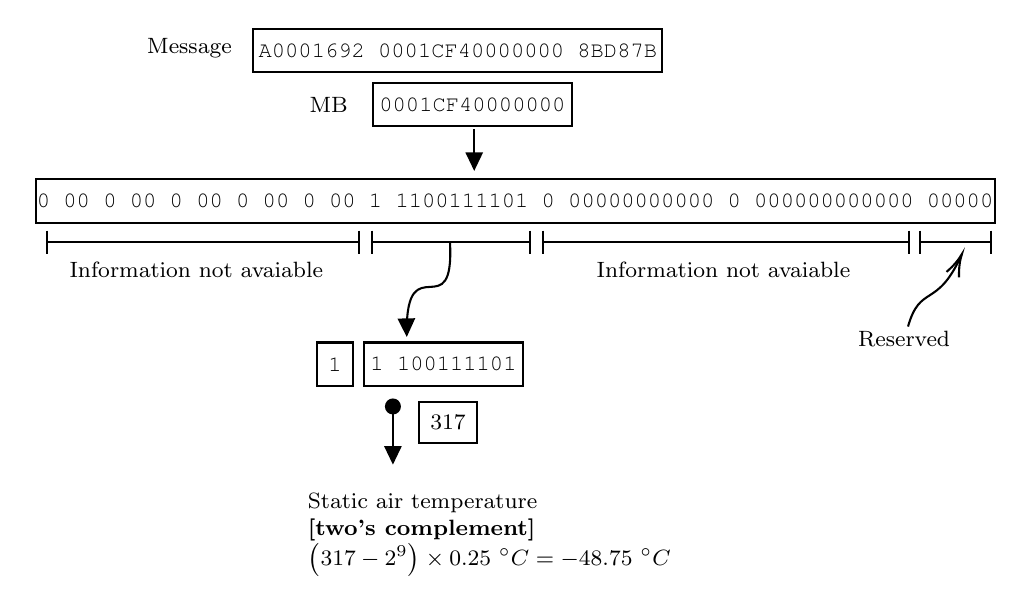
\begin{tikzpicture}[x=0.75pt,y=0.75pt,yscale=-1,xscale=1]
%uncomment if require: \path (0,368); %set diagram left start at 0, and has height of 368

%Straight Lines [id:da4065588661974868] 
\draw [line width=0.75]    (182.67,117.33) -- (259,117.33) ;
\draw [shift={(259,117.33)}, rotate = 180] [color={rgb, 255:red, 0; green, 0; blue, 0 }  ][line width=0.75]    (0,5.59) -- (0,-5.59)   ;
\draw [shift={(182.67,117.33)}, rotate = 180] [color={rgb, 255:red, 0; green, 0; blue, 0 }  ][line width=0.75]    (0,5.59) -- (0,-5.59)   ;
%Straight Lines [id:da8606101743392234] 
\draw [line width=0.75]    (265,117.33) -- (441.5,117.33) ;
\draw [shift={(441.5,117.33)}, rotate = 180] [color={rgb, 255:red, 0; green, 0; blue, 0 }  ][line width=0.75]    (0,5.59) -- (0,-5.59)   ;
\draw [shift={(265,117.33)}, rotate = 180] [color={rgb, 255:red, 0; green, 0; blue, 0 }  ][line width=0.75]    (0,5.59) -- (0,-5.59)   ;
%Curve Lines [id:da10322788127976112] 
\draw    (220.33,117.33) .. controls (222.46,159.15) and (199.45,118.69) .. (199.47,160.35) ;
\draw [shift={(199.5,163)}, rotate = 268.75] [fill={rgb, 255:red, 0; green, 0; blue, 0 }  ][line width=0.08]  [draw opacity=0] (8.93,-4.29) -- (0,0) -- (8.93,4.29) -- cycle    ;
%Straight Lines [id:da8466832782097071] 
\draw    (232,63) -- (232,80) ;
\draw [shift={(232,83)}, rotate = 270] [fill={rgb, 255:red, 0; green, 0; blue, 0 }  ][line width=0.08]  [draw opacity=0] (8.93,-4.29) -- (0,0) -- (8.93,4.29) -- cycle    ;
%Straight Lines [id:da4977418628626593] 
\draw    (192.83,196.5) -- (192.83,221.5) ;
\draw [shift={(192.83,224.5)}, rotate = 270] [fill={rgb, 255:red, 0; green, 0; blue, 0 }  ][line width=0.08]  [draw opacity=0] (8.93,-4.29) -- (0,0) -- (8.93,4.29) -- cycle    ;
\draw [shift={(192.83,196.5)}, rotate = 90] [color={rgb, 255:red, 0; green, 0; blue, 0 }  ][fill={rgb, 255:red, 0; green, 0; blue, 0 }  ][line width=0.75]      (0, 0) circle [x radius= 3.35, y radius= 3.35]   ;
%Straight Lines [id:da5955016490623266] 
\draw [line width=0.75]    (26,117.33) -- (176.5,117.33) ;
\draw [shift={(176.5,117.33)}, rotate = 180] [color={rgb, 255:red, 0; green, 0; blue, 0 }  ][line width=0.75]    (0,5.59) -- (0,-5.59)   ;
\draw [shift={(26,117.33)}, rotate = 180] [color={rgb, 255:red, 0; green, 0; blue, 0 }  ][line width=0.75]    (0,5.59) -- (0,-5.59)   ;
%Straight Lines [id:da5052935437984565] 
\draw [line width=0.75]    (446.67,117.33) -- (481,117.33) ;
\draw [shift={(481,117.33)}, rotate = 180] [color={rgb, 255:red, 0; green, 0; blue, 0 }  ][line width=0.75]    (0,5.59) -- (0,-5.59)   ;
\draw [shift={(446.67,117.33)}, rotate = 180] [color={rgb, 255:red, 0; green, 0; blue, 0 }  ][line width=0.75]    (0,5.59) -- (0,-5.59)   ;
%Curve Lines [id:da0284439343230396] 
\draw    (441,158) .. controls (446.88,137.42) and (454.68,149.49) .. (466.28,124.57) ;
\draw [shift={(467,123)}, rotate = 473.96] [color={rgb, 255:red, 0; green, 0; blue, 0 }  ][line width=0.75]    (10.93,-3.29) .. controls (6.95,-1.4) and (3.31,-0.3) .. (0,0) .. controls (3.31,0.3) and (6.95,1.4) .. (10.93,3.29)   ;

% Text Node
\draw    (125.63,14.5) -- (322.63,14.5) -- (322.63,35.5) -- (125.63,35.5) -- cycle  ;
\draw (224.13,25) node  [font=\footnotesize] [align=left] {{\fontfamily{pcr}\selectfont A0001692 0001CF40000000 8BD87B}};
% Text Node
\draw (161.88,51) node  [font=\footnotesize] [align=left] {MB};
% Text Node
\draw    (20.7,87) -- (482.7,87) -- (482.7,108) -- (20.7,108) -- cycle  ;
\draw (251.7,97.5) node  [font=\footnotesize] [align=left] {{\fontfamily{pcr}\selectfont 0 00 0 00 0 00 0 00 0 00 1 1100111101 0 00000000000 0 000000000000 00000}};
% Text Node
\draw    (183.13,40.5) -- (279.13,40.5) -- (279.13,61.5) -- (183.13,61.5) -- cycle  ;
\draw (231.13,51) node  [font=\footnotesize] [align=left] {{\fontfamily{pcr}\selectfont 0001CF40000000}};
% Text Node
\draw (94.82,24) node  [font=\footnotesize] [align=left] {Message};
% Text Node
\draw    (156.38,165.67) -- (173.38,165.67) -- (173.38,186.67) -- (156.38,186.67) -- cycle  ;
\draw (164.88,176.17) node  [font=\footnotesize] [align=left] {{\fontfamily{pcr}\selectfont 1}};
% Text Node
\draw    (178.7,165.67) -- (255.7,165.67) -- (255.7,186.67) -- (178.7,186.67) -- cycle  ;
\draw (217.2,176.17) node  [font=\footnotesize] [align=left] {{\fontfamily{pcr}\selectfont 1 100111101}};
% Text Node
\draw    (205.42,194.25) -- (233.42,194.25) -- (233.42,214.25) -- (205.42,214.25) -- cycle  ;
\draw (219.42,204.25) node  [font=\footnotesize] [align=left] {317};
% Text Node
\draw (239.26,258.5) node  [font=\footnotesize] [align=left] {Static air temperature\\\textbf{[two's complement]}\\$\displaystyle \left( 317-2^{9}\right) \times 0.25\ ^{\circ } C=-48.75\ ^{\circ } C$};
% Text Node
\draw (352.09,130.83) node  [font=\footnotesize] [align=left] {Information not avaiable};
% Text Node
\draw (98.09,130.83) node  [font=\footnotesize] [align=left] {Information not avaiable};
% Text Node
\draw (439.09,163.83) node  [font=\footnotesize] [align=left] {Reserved};


\end{tikzpicture}

  \caption{Meteorological harzard report (BDS 4,5) decoding example}
  \label{fig:bds45_example}
\end{figure}


\begin{notebox}{Note}
The availability of BDS 4,4 messages is quite low. Very few aircraft's transponders have these capabilities enabled. BDS 4,5 message is even rarer. When a message is transmitted, it is very common that information in many fields are not available.
\end{notebox}

